\documentclass[border=10pt]{standalone}

%%% Pakete %%%
\usepackage[utf8]{inputenc}
\usepackage[english]{babel}
\usepackage{tikz} 
\usetikzlibrary{er,positioning}

\begin{document}

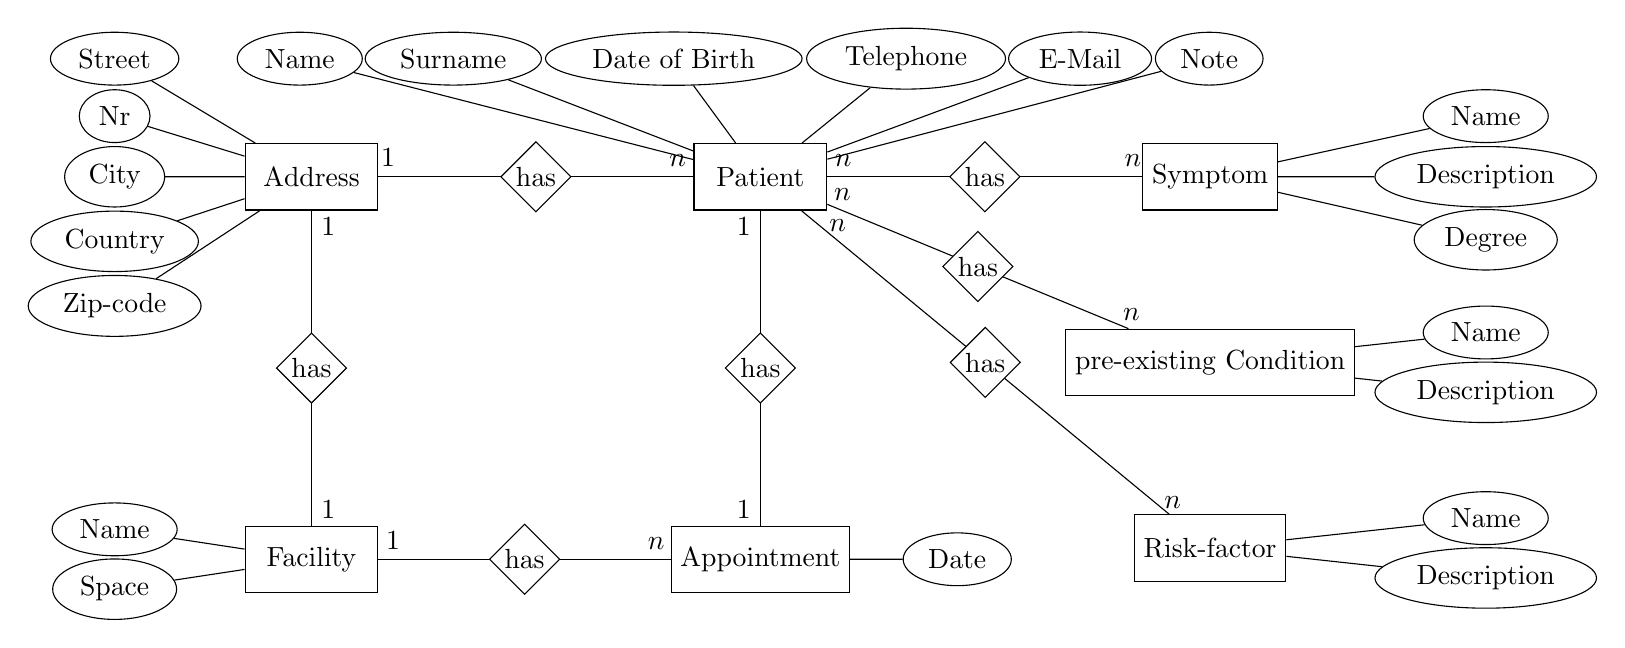
\begin{tikzpicture}[node distance=4cm, every edge/.style={link}]

    \node[entity] (patient) {Patient}
    [grow=up, sibling distance=3cm, align=center]
    child {node[attribute, xshift=-1.8cm] {Note}}
    child {node[attribute, xshift=-4.4mm] {E-Mail}}
    child {node[attribute, xshift=3.5mm] {Telephone}}
    child {node[attribute, xshift=4mm] {Date of Birth}}
    child {node[attribute, xshift=0.6cm] {Surname}}
    child {node[attribute, xshift=1.65cm] {Name}};

    \node[entity] (symptom) [right = of patient] {Symptom}
    [grow=right]
    child {node[attribute, xshift=2cm, yshift=0.7cm] {Degree}}
    child {node[attribute, xshift=2cm, yshift=0mm] {Description}}
    child {node[attribute, xshift=2cm, yshift=-0.73cm] {Name}};

    \node[entity] (condition) [below = of symptom, yshift=2.5cm] {pre-existing Condition}
    [grow=right]
    child {node[attribute, xshift=2cm, yshift=0.37cm] {Description}}
    child {node[attribute, xshift=2cm, yshift=-0.37cm] {Name}};

    \node[entity] (risk) [below = of condition, yshift=2.5cm] {Risk-factor}
    [grow=right]
    child {node[attribute, xshift=2cm, yshift=0.37cm] {Description}}
    child {node[attribute, xshift=2cm, yshift=-0.37cm] {Name}};

    \node[entity] (address) [left = of patient] {Address}
    [grow=left]
    child {node[attribute, xshift=-1cm, yshift=-1.5cm] {Street}}
    child {node[attribute, xshift=-1cm, yshift=-0.73cm] {Nr}}
    child {node[attribute, xshift=-1cm, yshift=0cm] {City}}
    child {node[attribute, xshift=-1cm, yshift=0.68cm] {Country}}
    child {node[attribute, xshift=-1cm, yshift=1.36cm] {Zip-code}};

    \node[entity] (facility) [below = of address] {Facility}
    [grow=left]
    child {node[attribute, xshift=-1cm, yshift=-0.37cm] {Name}}
    child {node[attribute, xshift=-1cm, yshift=0.37cm] {Space}};


    \node[entity] (appointment) [below = of patient] {Appointment}
    [grow=right]
    child {node[attribute, xshift=1cm] {Date}};

    \draw (patient) -- node [relationship, fill=white!100] {has} (symptom)
    node[pos=0.05, above]{$n$} node[pos=0.97, above]{$n$};

    \draw (patient) -- node [relationship, fill=white!100] {has} (condition)
    node[pos=0.05, above]{$n$} node[pos=1.01, above]{$n$};

    \draw (patient) -- node [relationship, fill=white!100] {has} (risk)
    node[pos=0.05, right]{$n$} node[pos=0.96, right]{$n$};

    \draw (patient) -- node [relationship, fill=white!100] {has} (appointment)
    node[pos=0.05, left]{$1$} node[pos=0.95, left]{$1$};

    \draw (patient) -- node [relationship, fill=white!100] {has} (address)
    node[pos=0.05, above]{$n$} node[pos=0.97, above]{$1$};

    \draw (facility) -- node [relationship, fill=white!100] {has} (address)
    node[pos=0.05, right]{$1$} node[pos=0.95, right]{$1$};

    \draw (facility) -- node [relationship, fill=white!100] {has} (appointment)
    node[pos=0.05, above]{$1$} node[pos=0.95, above]{$n$};

\end{tikzpicture}

\end{document}
